\documentclass[twocolumn]{article}
\usepackage{graphicx}
\usepackage{float}
\usepackage{placeins}
\usepackage[dutch,english]{babel}
\usepackage{geometry}
\geometry{margin=1in}
\usepackage{abstract}
\renewcommand{\abstractnamefont}{\normalfont\Large\bfseries} % Abstract title font
\renewcommand{\abstracttextfont}{\normalfont} % Abstract text font
\usepackage{titlesec}
\usepackage{hyperref}

\title{Multi-Splat-representaties: segmentatie en objectmanipulatie in Gaussiaanse splatting}
\author{Bavo Verstraeten\\
	Promotors: Prof. dr. Peter Lambert, Prof. dr. ir. Glenn Van Wallendael}

\begin{document}
	\selectlanguage{dutch}
	\pagenumbering{gobble}
\twocolumn[
\maketitle
\begin{onecolabstract}
	\noindent
Gaussiaanse splatting is een innovatieve techniek voor het real-time renderen van complexe scènes. Deze masterproef verbetert de bruikbaarheid en nauwkeurigheid van Gaussiaanse splats in de Unity-engine door een bestaande open-source Unity-extensie uit te breiden. De studie richt zich op twee centrale uitdagingen. Allereerst leidde de oorspronkelijke Unity-extensie tot visuele artefacten bij overlappende \linebreak splat-objecten, omdat de sortering en rendering per GameObject gebeurde. Dit probleem werd opgelost door de renderingspipeline aan te passen, zodat een globale sortering per splat wordt uitgevoerd. Hierdoor wordt de correcte dieptevolgorde in de volledige scène gegarandeerd. Ten tweede vereist de voorbereiding van splats voor animatie in Unity traditioneel handmatige en foutgevoelige segmentatie. Om dit proces te vergemakkelijken, werd een semi-automatische segmentatiepipeline ontwikkeld door de tools SAM, SAM2 en SAGD te combineren. Deze aanpak automatiseert een groot deel van het segmentatieproces, terwijl gebruikerscontrole voor verfijning en correctie behouden blijft. Dit resulteert in hiërarchisch opgebouwde GameObjects, gebaseerd op splat-data. Deze bijdragen verbeteren zowel de visuele kwaliteit van de rendering als de efficiëntie van de workflow, en bevorderen de integratie van Gaussiaanse splatting in real-time interactieve toepassingen.
\end{onecolabstract}
\vspace{1cm}
]
	
	\section{Introductie}
De afgelopen jaren heeft het vakgebied van real-time 3D-rendering een verschuiving doorgemaakt van traditionele, op geometrie gebaseerde representaties naar puntgebaseerde methoden die complexere details in scènes beter vastleggen. Binnen deze ontwikkeling heeft Gaussiaanse splatting \cite{OriginalSplatting} zich ontwikkeld tot een veelbelovend alternatief. Deze techniek maakt het mogelijk om fotorealistische scènes in real-time weer te geven door oppervlakken te representeren als verzamelingen van ruimtelijk verspreide Gaussiaanse functies. In tegenstelling tot neurale netwerkbenaderingen zoals Neural Radiance Fields (NeRF) \cite{Nerf}, vermijdt Gaussiaanse splatting de noodzaak van kostbare netwerkqueries, waardoor het bijzonder geschikt is voor interactieve toepassingen waar prestaties cruciaal zijn.
\\\\
Het toepassen van Gaussiaanse splatting in real-time engines zoals Unity brengt echter specifieke uitdagingen met zich mee. De bestaande open-source implementatie \cite{Aras} is functioneel, maar vertoont beperkingen wanneer ze wordt ingezet in dynamische of interactieve omgevingen. Met name problemen met diepte-rendering en handmatige segmentatieworkflows belemmeren een naadloze integratie van deze veelbelovende techniek in gebruikelijke productieprocessen.
\\\\
Dit werk onderzoekt deze uitdagingen in detail, identificeert belangrijke knelpunten en stelt concrete oplossingen voor die zowel de visuele kwaliteit als de bruikbaarheid van Gaussiaanse splats in Unity verbeteren. Door te focussen op zowel de renderarchitectuur als het segmentatieproces, beoogt deze studie de kloof te overbruggen tussen academische vooruitgang op het gebied van puntgebaseerde rendering en de praktische inzet ervan in real-time interactieve systemen.
	\section{Methodologie}
	\subsection{Globale per-splat sortering}
De Unity-extensie past een sortering per GameObject toe, wat inhoudt dat bij twee GameObjects het ene altijd volledig voor het andere wordt weergegeven. Deze methode is geschikt voor eenvoudige scènes, maar leidt tot render-fouten in complexere gevallen.
\\\\
Om dit probleem te verhelpen, is de renderer aangepast om een globale per-splat sortering te implementeren. In plaats van elk GameObject een eigen grafische buffer toe te wijzen voor de verwerkte splatgegevens, werd één globale buffer ingevoerd. De compute shader van elk object schrijft direct in deze buffer, waardoor de splatgegevens van alle objecten efficiënt worden samengevoegd. Zodra de globale buffer gevuld is, wordt deze gesorteerd en gerenderd op basis van de werkelijke diepte van elke splat. Dit levert correcte en consistente visuele resultaten op, zonder onnodige complexiteit.	
	\subsection{Segmentatie-Pipeline}
De Unity-extensie bevat een ingebouwde tool om handmatig segmenten van een Gaussiaanse Splat te isoleren. Deze methode wordt echter steeds omslachtiger en minder efficiënt bij het werken met grote of complexe segmenten, waardoor geautomatiseerde ondersteuning zeer gewenst is. Automatische segmentatie begint meestal met een image mask, en van de verschillende methoden die in de literatuur zijn onderzocht, bleek SAGD \cite{SAGD} bijzonder geschikt. SAGD introduceert Gaussiaanse decompositie, een proces waarbij splats langs de rand van de mask worden gesplitst. Dit zorgt voor vloeiendere segmentranden en lost het probleem op van grote, chaotische interne splats die vaak voorkomen in Gaussiaanse Splat-modellen.
\\\\
SAGD ondervindt uitdagingen bij het omzetten van een 2D image masks naar een nauwkeurig 3D splat mask. Om deze beperkingen te overwinnen, zijn SAM \cite{SAM} en SAM2 \cite{SAM2} geïntegreerd in de segmentatie-pipeline. SAM2 maakt segmentatie van videobeelden mogelijk, waardoor masks vanuit meerdere hoeken kunnen worden gegenereerd wanneer vloeiende trainingsdata beschikbaar is. SAM, dat zich enkel richt op beeldsegmentatie, biedt een veelzijdige reeks tools die zowel SAM2 als SAGD aanvullen.
\\\\
Deze drie tools – SAM, SAM2 en SAGD – vormen samen een flexibele segmentatie-pipeline die meerdere niveaus van automatisering ondersteunt. De gebruiker kan ervoor kiezen om hiërarchische aanwijzingen te geven voor nauwkeurige segmentatie, gebruik te maken van automatische hiërarchiebepaling om handmatige input te verminderen, of het systeem volledige segmentatie te laten uitvoeren zonder enige tussenkomst.
	\section{Resultaten}
Figuur~\ref{fig:render} illustreert de render-fouten die optreden bij per-GameObject sortering, evenals de verbeteringen die worden bereikt met globale per-splat sortering. De arm van de bulldozer, die als afzonderlijk GameObject is geïmplementeerd, vormt een uitdaging voor per-GameObject sortering. In de linkerafbeelding zijn de pompen op de arm niet zichtbaar. In de rechterafbeelding is een deel van het voorste gedeelte van de bulldozer verdwenen. De onderste afbeelding toont de gecorrigeerde weergave die wordt verkregen met globale per-splat sortering, waarbij de diepte van elke splat globaal wordt geëvalueerd. Hierdoor worden deze render-fouten opgelost en blijft de visuele samenhang van het model behouden.


	\begin{figure}[h!]
		\centering
		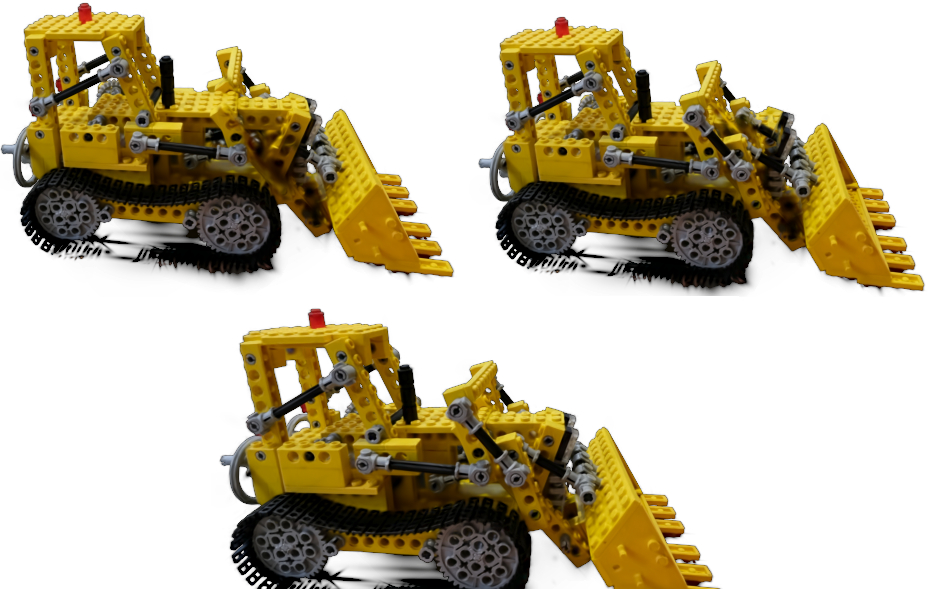
\includegraphics[width=0.5\textwidth]{Images/Untitled.png}
		\caption{Onjuiste weergave als gevolg van per-GameObject sortering (links, rechts). Correcte weergave met globale per-splat sortering (onder).}
		\label{fig:render}
	\end{figure}
	\FloatBarrier
	\noindent
Figuur~\ref{fig:trucks} toont de segmentatieprestaties van de ontwikkelde pipeline, die drie verschillende algoritmes combineert om uiteenlopende niveaus van automatisering en controle te bieden. De bovenste afbeelding illustreert volledig automatische segmentatie, waarbij het vrachtwagenmodel zonder enige gebruikersinvoer in meerdere segmenten wordt opgedeeld. De rechterafbeelding laat de semi-automatische benadering zien, waarbij met één enkel positief punt zowel de vrachtwagen van de omliggende scène wordt geïsoleerd als het houten platform van de vrachtwagen zelf wordt gescheiden. Deze methode vereist minimale invoer maar biedt beperkte controle over het resultaat. Hoewel niet afgebeeld, ondersteunt de pipeline ook een semi-automatische methode met volledige gebruikerssturing, waarbij de gebruiker hiërarchische aanwijzingen kan definiëren en het segmentatieproces naar wens kan sturen, wat nauwkeurige extractie van willekeurige segmentcombinaties in de scène mogelijk maakt. Hoewel de resultaten niet zonder onvolkomenheden zijn, staan deze algoritmes niet in concurrentie; in plaats daarvan vullen ze elkaar aan en blinkt elk uit onder specifieke omstandigheden.
	\begin{figure}[h!]
		\centering
		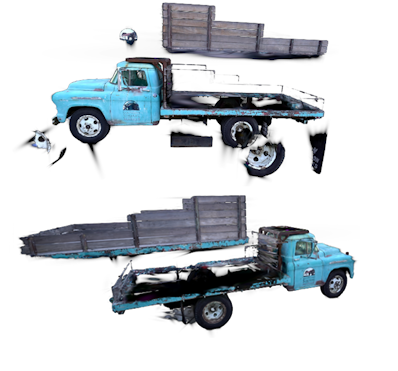
\includegraphics[width=0.5\textwidth]{Images/trucks.png}
		\caption{Segmentatie van een vrachtwagenmodel: volledig automatisch (boven) en semi-automatisch met een enkel gegeven punt (onder).
		}
		\label{fig:trucks}
	\end{figure}
	\FloatBarrier
	\noindent
	\section{Discussie}
Dit werk behandelt een belangrijke uitdaging bij de integratie van Gaussiaanse splats in de Unity-engine door een kritisch render-probleem op te lossen dat verband houdt met de sortering van splats. Door de introductie van een globale sorteringsmechanisme is de correctheid van de renderpipeline aanzienlijk verbeterd, wat ervoor zorgt dat splat-gebaseerde scènes zonder artefacten worden weergegeven, zelfs in complexe interactieve omgevingen. De verbeterde pipeline vergroot de bruikbaarheid van de bestaande open-source Unity-extensie en biedt onderzoekers en ontwikkelaars een robuuster hulpmiddel om splats te verkennen en te manipuleren. Deze vooruitgang wordt verwacht brede toepassingen in real-time rendering mogelijk te maken en het gebruik van Gaussiaanse splatting technieken verder te stimuleren.
\\\\
Een belangrijke bijdrage van deze thesis is de innovatieve combinatie van Gaussiaanse decompositie met een consistentere en betrouwbaardere mask-generatie vanuit meerdere perspectieven. Deze verbetering vergroot de toepasbaarheid van decompositie-gebaseerde segmentatie op steeds complexere scènes. Daarnaast verhoogt de introductie van meerdere niveaus van automatisering binnen de segmentatieworkflow de bruikbaarheid en biedt het flexibele oplossingen voor diverse segmentatietaken.
\\\\
Desondanks blijven er enkele beperkingen bestaan. Het volledig automatische segmentatie-algoritme genereert soms onzinnige segmenten, met name in scènes met hoge complexiteit of occlusie. Bovendien heeft het toepassen van Gaussiaanse decompositie op grote en complexe scènes geleid tot geheugenallocatiefouten, wat wijst op beperkingen in de schaalbaarheid. Daarnaast introduceert de afhankelijkheid van een vloeiende trainingsvideo voor SAM2 een beperking op het type modellen dat kan worden verwerkt, wat de algemene toepasbaarheid van het systeem vermindert.
\\
De richting voor toekomstig onderzoek is duidelijk. Een veelbelovende mogelijkheid is het simuleren van een bewegende camera binnen Unity om continue videoinvoer voor SAM2 te genereren. Verbeteringen in strategieën voor het combineren van masks kunnen ook leiden tot betrouwbaardere en preciezere segmentaties. Bovendien kan het integreren van informatie over de driedimensionale posities en structuren van splats – die in dit werk nog onderbenut blijven – de kwaliteit en stabiliteit van de segmentatie verbeteren, vooral in dichte of geoccludeerde scènes.


	\section{Conclusie}
Door kritieke beperkingen in zowel rendering als segmentatie aan te pakken, levert dit werk een significante bijdrage aan de praktische integratie van Gaussiaanse splatting in real-time toepassingen. De ontwikkelde oplossingen verbeteren niet alleen de visuele kwaliteit en workflow-efficiëntie in Unity, maar effenen ook het pad voor toekomstig onderzoek naar gedetailleerde, puntgebaseerde scene-representaties en hun toepassingen in interactieve systemen. Deze bijdragen vormen een betekenisvolle stap richting het realiseren van het volledige potentieel van Gaussiaanse splatting in complexe, dynamische omgevingen.


\bibliographystyle{IEEEtran}
\bibliography{references}

\end{document}
